%% ============================================================
%% Rapport de Projet – Infrastructures pour le Cloud et Big Data
%% Master M1/M2 – ENSEEIHT / INP Toulouse
%% ============================================================
\documentclass[12pt,a4paper,french]{report}

%% ── Encodage & langue ─────────────────────────────────────
\usepackage[utf8]{inputenc}
\usepackage[T1]{fontenc}
\usepackage{babel}

%% ── Mise en page ──────────────────────────────────────────
\usepackage[top=2.5cm, bottom=2.5cm, left=3cm, right=2.5cm]{geometry}
\usepackage{setspace}
\onehalfspacing

%% ── Typographie ──────────────────────────────────────────
\usepackage{lmodern}
\usepackage{microtype}

%% ── Couleurs & graphiques ─────────────────────────────────
\usepackage[dvipsnames,svgnames]{xcolor}
\usepackage{graphicx}
\usepackage{float}
\usepackage{tikz}
\usetikzlibrary{shapes.geometric, arrows.meta, positioning, fit, calc}

%% ── Listings (code) ───────────────────────────────────────
\usepackage{listings}
\usepackage{lstautogobble}

\definecolor{codebg}{HTML}{F8F8F8}
\definecolor{codeframe}{HTML}{CCCCCC}
\definecolor{keywordcolor}{HTML}{0000CC}
\definecolor{commentcolor}{HTML}{006600}
\definecolor{stringcolor}{HTML}{CC0000}
\definecolor{numbercolor}{HTML}{888888}

\lstdefinestyle{bash}{
  language=bash,
  backgroundcolor=\color{codebg},
  frame=single,
  rulecolor=\color{codeframe},
  basicstyle=\ttfamily\small,
  keywordstyle=\color{keywordcolor}\bfseries,
  commentstyle=\color{commentcolor}\itshape,
  stringstyle=\color{stringcolor},
  numberstyle=\tiny\color{numbercolor},
  numbers=left,
  numbersep=8pt,
  breaklines=true,
  breakatwhitespace=true,
  showstringspaces=false,
  tabsize=2,
  autogobble=true,
  xleftmargin=15pt,
  xrightmargin=5pt,
}

\lstdefinestyle{yaml}{
  language=Python,
  backgroundcolor=\color{codebg},
  frame=single,
  rulecolor=\color{codeframe},
  basicstyle=\ttfamily\footnotesize,
  keywordstyle=\color{keywordcolor}\bfseries,
  commentstyle=\color{commentcolor}\itshape,
  stringstyle=\color{stringcolor},
  numbers=left,
  numberstyle=\tiny\color{numbercolor},
  numbersep=8pt,
  breaklines=true,
  showstringspaces=false,
  tabsize=2,
  autogobble=true,
  xleftmargin=15pt,
}

\lstdefinestyle{python}{
  language=Python,
  backgroundcolor=\color{codebg},
  frame=single,
  rulecolor=\color{codeframe},
  basicstyle=\ttfamily\small,
  keywordstyle=\color{keywordcolor}\bfseries,
  commentstyle=\color{commentcolor}\itshape,
  stringstyle=\color{stringcolor},
  numberstyle=\tiny\color{numbercolor},
  numbers=left,
  numbersep=8pt,
  breaklines=true,
  showstringspaces=false,
  tabsize=4,
  autogobble=true,
  xleftmargin=15pt,
}

%% ── Hyperliens & PDF ──────────────────────────────────────
\usepackage[hidelinks,
  pdfauthor={Prénom NOM1, Prénom NOM2},
  pdftitle={Projet Infrastructure Cloud \& Big Data 2026},
  pdfsubject={Kubernetes, Prometheus, Spark sur GCP}
]{hyperref}

%% ── Tableaux ─────────────────────────────────────────────
\usepackage{booktabs}
\usepackage{tabularx}
\usepackage{multirow}
\usepackage[table]{xcolor}

%% ── Listes ───────────────────────────────────────────────
\usepackage{enumitem}

%% ── En-têtes et pieds de page ────────────────────────────
\usepackage{fancyhdr}
\pagestyle{fancy}
\fancyhf{}
\fancyhead[L]{\small\textit{Projet Cloud \& Big Data 2026}}
\fancyhead[R]{\small\textit{\leftmark}}
\fancyfoot[C]{\thepage}
\renewcommand{\headrulewidth}{0.4pt}

%% ── Boîtes colorées ──────────────────────────────────────
\usepackage{tcolorbox}
\tcbuselibrary{skins,breakable}

\newtcolorbox{notebox}[1][Note]{
  colback=blue!5!white, colframe=blue!50!black,
  title=#1, fonttitle=\bfseries,
  breakable
}
\newtcolorbox{warnbox}[1][Attention]{
  colback=orange!10!white, colframe=orange!80!black,
  title=#1, fonttitle=\bfseries,
  breakable
}
\newtcolorbox{resultbox}[1][Résultat]{
  colback=green!5!white, colframe=green!50!black,
  title=#1, fonttitle=\bfseries,
  breakable
}

%% ── Macro utiles ─────────────────────────────────────────
\newcommand{\cmd}[1]{\texttt{\small\color{keywordcolor}#1}}
\newcommand{\kw}[1]{\textbf{#1}}
\newcommand{\todo}[1]{\textcolor{red}{\textbf{[TODO: #1]}}}

%% ── Table des matières ───────────────────────────────────
\setcounter{tocdepth}{2}
\setcounter{secnumdepth}{3}

%% ════════════════════════════════════════════════════════════
\begin{document}

%% ── PAGE DE GARDE ─────────────────────────────────────────
\begin{titlepage}
  \centering
  \vspace*{1cm}
  
  {\Large\bfseries Institut National Polytechnique de Toulouse\\
  ENSEEIHT – Département Informatique et Mathématiques Appliquées}
  
  \vspace{0.5cm}
  \rule{\linewidth}{0.4pt}
  \vspace{1.5cm}
  
  {\Huge\bfseries Projet d'Infrastructure\\[0.3em]
  pour le Cloud et le Big Data}
  
  \vspace{0.8cm}
  
  {\Large\itshape Déploiement de Kubernetes, Prometheus et Apache Spark\\
  sur Google Cloud Platform}
  
  \vspace{1.5cm}
  \rule{\linewidth}{0.4pt}
  \vspace{1.5cm}
  
  \begin{minipage}{0.45\textwidth}
    \centering
    {\large\bfseries Auteurs}\\[0.4em]
    Prénom \textsc{Nom1}\\
    Prénom \textsc{Nom2}
  \end{minipage}
  \hfill
  \begin{minipage}{0.45\textwidth}
    \centering
    {\large\bfseries Encadrant}\\[0.4em]
    Boris \textsc{Teabe}\\[0.8em]
    {\large\bfseries Année universitaire}\\[0.4em]
    2025 -- 2026
  \end{minipage}
  
  \vfill
  {\large UE~: Infrastructures pour le Cloud et le Big Data\\
  Master 1 -- Informatique}
  
  \vspace{0.5cm}
  {\large\bfseries \today}
\end{titlepage}

%% ── RÉSUMÉ ────────────────────────────────────────────────
\begin{abstract}
\noindent
Ce rapport présente le travail réalisé dans le cadre du projet de l'UE \emph{Infrastructures pour le Cloud et le Big Data}. L'objectif est de déployer et d'opérer une infrastructure complète de traitement distribué des données en tirant parti des technologies modernes du Cloud et de l'orchestration de conteneurs.

Le projet se décompose en trois phases techniques~: (1) le déploiement d'un cluster \kw{Kubernetes} sur des machines virtuelles hébergées sur \kw{Google Cloud Platform} (GCP)~; (2) l'instrumentation de ce cluster avec \kw{Prometheus} et \kw{Grafana} pour le monitoring des ressources~; (3) le déploiement d'\kw{Apache Spark} en mode cluster et l'exécution de l'application de référence \kw{WordCount} avec collecte de métriques.

L'ensemble de l'infrastructure est défini sous forme de code (\emph{Infrastructure as Code}), ce qui garantit sa reproductibilité. Ce rapport détaille les choix d'architecture, les configurations mises en \oe{}uvre et les observations tirées des expérimentations.

\medskip
\noindent\textbf{Mots-clés~:} Kubernetes, GCP, Prometheus, Grafana, Apache Spark, Big Data, WordCount, conteneurisation, monitoring, Infrastructure as Code.
\end{abstract}

\tableofcontents
\listoffigures
\listoftables
\clearpage

%% ════════════════════════════════════════════════════════════
\chapter{Introduction}
%% ════════════════════════════════════════════════════════════

\section{Contexte et motivations}

L'essor du \kw{Big Data} a profondément modifié les pratiques du génie logiciel et des systèmes distribués. Les organisations traitent aujourd'hui des volumes de données de l'ordre du pétaoctet, ce qui rend obsolètes les architectures monolithiques traditionnelles. Deux paradigmes ont émergé pour répondre à ces défis~: l'\kw{orchestration de conteneurs} via Kubernetes, et les \kw{moteurs de traitement distribué} tels qu'Apache Spark.

Dans ce contexte, ce projet vise à consolider les compétences acquises lors des travaux pratiques du cours en réalisant une infrastructure de bout en bout~: depuis la création des machines virtuelles sur le Cloud public jusqu'à l'exécution d'une application de traitement de données à grande échelle, en passant par la mise en place d'un système de monitoring de production.

\section{Périmètre du projet}

Le projet couvre les quatre axes suivants~:

\begin{enumerate}[leftmargin=*]
  \item \textbf{Déploiement de Kubernetes sur GCP}~: création d'un cluster de machines virtuelles sur Google Cloud Platform et configuration d'un cluster Kubernetes à la main (\emph{kubeadm}), par opposition aux services gérés comme GKE.
  
  \item \textbf{Monitoring avec Prometheus et Grafana}~: déploiement d'une pile de monitoring complète permettant de visualiser l'utilisation CPU et mémoire des pods et nœuds en temps réel.
  
  \item \textbf{Apache Spark sur Kubernetes}~: déploiement de Spark en mode cluster (1 master, 2 workers) et exécution de l'application WordCount avec collecte des métriques d'exécution.
  
  \item \textbf{Rédaction du rapport}~: documentation des choix techniques, des procédures de déploiement et des résultats obtenus.
\end{enumerate}

\section{Organisation du travail}

\begin{table}[H]
\centering
\caption{Répartition des tâches entre les membres du groupe}
\label{tab:repartition}
\begin{tabularx}{\textwidth}{lXX}
\toprule
\textbf{Phase} & \textbf{Membre 1} & \textbf{Membre 2} \\
\midrule
Phase 1 – GCP \& Kubernetes & Configuration GCP, scripts shell & Installation kubeadm, réseau Flannel \\
\addlinespace
Phase 2 – Monitoring & Déploiement Prometheus & Configuration Grafana, dashboards \\
\addlinespace
Phase 3 – Spark & Déploiement Spark/K8s & Application WordCount, métriques \\
\addlinespace
Phase 4 – Rapport & Phases 1 et 2 & Phases 3, conclusion, relectures \\
\bottomrule
\end{tabularx}
\end{table}

\section{Structure du rapport}

Ce rapport suit la progression naturelle du projet. Le chapitre~\ref{chap:background} dresse un état de l'art des technologies utilisées. Les chapitres~\ref{chap:phase1}, \ref{chap:phase2} et~\ref{chap:phase3} détaillent respectivement chaque phase technique. Le chapitre~\ref{chap:conclusion} conclut et présente les perspectives.

%% ════════════════════════════════════════════════════════════
\chapter{État de l'art et technologies}
\label{chap:background}
%% ════════════════════════════════════════════════════════════

\section{L'orchestration de conteneurs}

\subsection{Docker et la conteneurisation}

La conteneurisation repose sur les mécanismes d'isolation du noyau Linux~: les \emph{namespaces} (isolation des processus, réseau, système de fichiers) et les \emph{cgroups} (limitation et comptabilité des ressources). Un \kw{conteneur} encapsule une application et toutes ses dépendances dans une image portable et reproductible.

Contrairement à la virtualisation complète (hyperviseur de type~1 ou~2), les conteneurs partagent le noyau hôte, ce qui les rend nettement plus légers en termes de surcoût mémoire et de temps de démarrage (typiquement inférieur à la seconde).

\subsection{Kubernetes : architecture et concepts clés}

\kw{Kubernetes} (K8s) est un orchestrateur de conteneurs open-source développé à l'origine par Google et maintenu par la Cloud Native Computing Foundation (CNCF). Son architecture distingue deux types de nœuds~:

\begin{description}
  \item[\emph{Control Plane} (nœud master)] gère l'état désiré du cluster via plusieurs composants~:
    \begin{itemize}
      \item \cmd{kube-apiserver}~: point d'entrée REST de toutes les opérations~;
      \item \cmd{etcd}~: base de données clé-valeur distribuée stockant l'état du cluster~;
      \item \cmd{kube-scheduler}~: planifie les pods sur les nœuds en fonction des ressources disponibles~;
      \item \cmd{kube-controller-manager}~: boucles de contrôle (ReplicaSet, Deployment, etc.).
    \end{itemize}
  
  \item[\emph{Worker nodes}] exécutent les charges de travail via~:
    \begin{itemize}
      \item \cmd{kubelet}~: agent qui s'assure que les conteneurs définis dans les pods sont bien lancés~;
      \item \cmd{kube-proxy}~: règles \texttt{iptables}/IPVS pour le routage réseau des services~;
      \item \emph{Container Runtime}~: \cmd{containerd} dans notre cas.
    \end{itemize}
\end{description}

Les \kw{objets Kubernetes} fondamentaux utilisés dans ce projet sont décrits dans le tableau~\ref{tab:k8s-objects}.

\begin{table}[H]
\centering
\caption{Objets Kubernetes utilisés dans le projet}
\label{tab:k8s-objects}
\rowcolors{2}{gray!10}{white}
\begin{tabularx}{\textwidth}{lX}
\toprule
\textbf{Objet} & \textbf{Rôle} \\
\midrule
\texttt{Pod} & Unité atomique d'exécution~: un ou plusieurs conteneurs partageant réseau et stockage \\
\texttt{Deployment} & Gère le cycle de vie des pods~; garantit le nombre de répliques désiré \\
\texttt{Service} & Expose un ensemble de pods via une IP stable et du load balancing \\
\texttt{ConfigMap} & Stocke des données de configuration non sensibles \\
\texttt{Namespace} & Partition logique du cluster pour isoler les charges de travail \\
\texttt{ServiceAccount} & Identité d'un pod pour interagir avec l'API Kubernetes \\
\texttt{ClusterRole/Binding} & Contrôle d'accès basé sur les rôles (RBAC) \\
\texttt{PersistentVolumeClaim} & Demande de stockage persistant \\
\bottomrule
\end{tabularx}
\end{table}

\section{Google Cloud Platform}

\kw{Google Cloud Platform} (GCP) est l'un des trois principaux fournisseurs de Cloud public avec AWS et Azure. Nous utilisons principalement le service \kw{Compute Engine} (équivalent EC2 d'AWS) pour créer nos machines virtuelles, ainsi que les \kw{VPC} (Virtual Private Cloud) pour l'isolation réseau.

Le choix de GCP s'explique par~: (i) la disponibilité de crédits gratuits pour les nouveaux comptes~; (ii) la présence d'une région en France (\texttt{europe-west9}, Paris)~; (iii) la richesse de l'outil CLI \cmd{gcloud}.

\section{Apache Spark}

\kw{Apache Spark} est un moteur de traitement distribué en mémoire, conçu pour surpasser Hadoop MapReduce en performance grâce au calcul in-memory. Son modèle de programmation repose sur les \kw{Resilient Distributed Datasets} (RDD), des collections immuables et partitionnées d'éléments pouvant être traitées en parallèle.

Spark supporte également une API haut niveau orientée \kw{DataFrame/Dataset}, optimisée par le compilateur Catalyst. Dans ce projet, nous utilisons les deux APIs pour illustrer les approches bas et haut niveau.

L'application \kw{WordCount} est le ``Hello World'' du Big Data~: elle compte le nombre d'occurrences de chaque mot dans un corpus de texte. Elle illustre parfaitement le paradigme \kw{MapReduce}~:
\begin{itemize}
  \item \textbf{Map}~: chaque ligne est découpée en mots, chaque mot émet le tuple \texttt{(mot, 1)}~;
  \item \textbf{Reduce}~: les tuples de même clé sont agrégés par somme.
\end{itemize}

\section{Monitoring~: Prometheus et Grafana}

\kw{Prometheus} est un système de monitoring et d'alerting open-source initialement développé par SoundCloud. Il suit un modèle de \emph{pull}~: il interroge (\emph{scrape}) régulièrement les endpoints \texttt{/metrics} exposés par les applications. Les métriques sont stockées dans une base de données de séries temporelles (TSDB) avec un modèle de données multi-dimensionnel (labels clé-valeur).

\kw{Grafana} est un outil de visualisation qui se connecte à Prometheus (et d'autres sources) pour afficher des tableaux de bord interactifs. La combinaison Prometheus~+~Grafana constitue le standard de facto du monitoring dans les environnements cloud-natifs.

%% ════════════════════════════════════════════════════════════
\chapter{Phase 1~: Déploiement de Kubernetes sur GCP}
\label{chap:phase1}
%% ════════════════════════════════════════════════════════════

\section{Architecture cible}

Nous déployons un cluster Kubernetes composé de deux nœuds~:
\begin{itemize}
  \item \textbf{k8s-master}~: nœud control plane (API server, scheduler, etcd, controller manager)~;
  \item \textbf{k8s-worker-1}~: nœud worker (kubelet, kube-proxy, containerd).
\end{itemize}

La figure~\ref{fig:arch-k8s} présente l'architecture générale de notre infrastructure.

\begin{figure}[H]
\centering
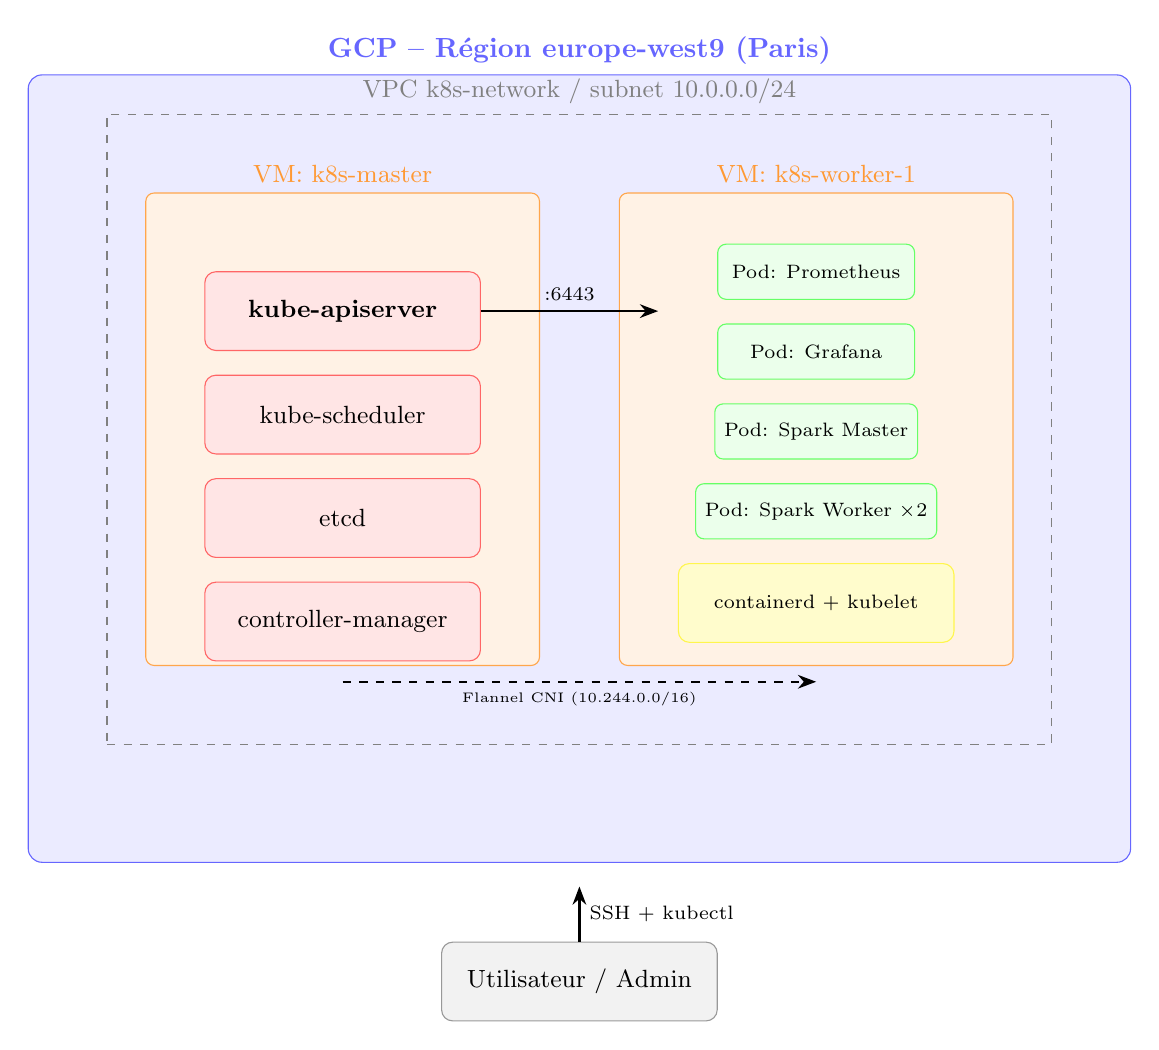
\begin{tikzpicture}[
  node distance=1.5cm and 2cm,
  box/.style={draw, rounded corners, minimum width=3.5cm, minimum height=1cm, 
               text centered, font=\small},
  gcp/.style={draw=blue!60, fill=blue!8, rounded corners=5pt},
  vm/.style={draw=orange!70, fill=orange!10, rounded corners=3pt},
  pod/.style={draw=green!60, fill=green!8, rounded corners=3pt, minimum width=2.5cm, minimum height=0.7cm, font=\scriptsize},
  arrow/.style={-Stealth, thick}
]

%% GCP Region
\node[gcp, minimum width=14cm, minimum height=10cm, label={[blue!60]above:\textbf{GCP – Région europe-west9 (Paris)}}] (gcp) {};

%% VPC
\node[draw=gray, dashed, minimum width=12cm, minimum height=8cm, below=0.5cm of gcp.north, 
      label={[gray]above:\small VPC k8s-network / subnet 10.0.0.0/24}] (vpc) {};

%% Master VM
\node[vm, minimum width=5cm, minimum height=6cm, 
      left=0.5cm of vpc.center, yshift=0,
      label={[orange!80]above:\small VM: k8s-master}] (master-vm) {};

\node[box, fill=red!10, draw=red!60] at ([yshift=1.5cm]master-vm.center) (api) {\textbf{kube-apiserver}};
\node[box, fill=red!10, draw=red!60, below=0.3cm of api] (sched) {kube-scheduler};
\node[box, fill=red!10, draw=red!60, below=0.3cm of sched] (etcd) {etcd};
\node[box, fill=red!10, draw=red!60, below=0.3cm of etcd] (ctrl) {controller-manager};

%% Worker VM
\node[vm, minimum width=5cm, minimum height=6cm,
      right=0.5cm of vpc.center, yshift=0,
      label={[orange!80]above:\small VM: k8s-worker-1}] (worker-vm) {};

\node[pod] at ([yshift=2cm]worker-vm.center) (pod1) {Pod: Prometheus};
\node[pod, below=0.3cm of pod1] (pod2) {Pod: Grafana};
\node[pod, below=0.3cm of pod2] (pod3) {Pod: Spark Master};
\node[pod, below=0.3cm of pod3] (pod4) {Pod: Spark Worker ×2};
\node[box, fill=yellow!20, draw=yellow!70, below=0.3cm of pod4, font=\scriptsize] (rt) {containerd + kubelet};

%% Arrows
\draw[arrow] (api) -- node[above, font=\scriptsize]{:6443} ([xshift=0.5cm]api.east -| worker-vm.west);
\draw[arrow, dashed] ([yshift=-0.2cm]master-vm.south) -- node[below, font=\tiny]{Flannel CNI (10.244.0.0/16)} ([yshift=-0.2cm]worker-vm.south);

%% External user
\node[box, below=2.5cm of vpc, draw=gray!80, fill=gray!10] (user) {\small Utilisateur / Admin};
\draw[arrow] (user) -- node[right, font=\scriptsize]{SSH + kubectl} ([yshift=-0.3cm]gcp.south);

\end{tikzpicture}
\caption{Architecture de l'infrastructure Kubernetes sur GCP}
\label{fig:arch-k8s}
\end{figure}

\section{Création des machines virtuelles sur GCP}

\subsection{Configuration du projet GCP}

Avant de créer les ressources, nous configurons l'outil CLI \cmd{gcloud} et définissons notre projet~:

\begin{lstlisting}[style=bash, caption={Initialisation de gcloud}]
# Installer gcloud SDK (https://cloud.google.com/sdk/docs/install)
gcloud init
gcloud auth login
gcloud config set project bigdata-projet-2026
gcloud config set compute/zone europe-west9-a
\end{lstlisting}

\subsection{Réseau VPC et règles de pare-feu}

Nous créons un réseau VPC dédié pour isoler notre cluster du reste des ressources GCP. Cette pratique est recommandée pour la sécurité et la gestion du trafic réseau.

\begin{lstlisting}[style=bash, caption={Création du VPC et des règles de firewall}]
# Créer le VPC
gcloud compute networks create k8s-network --subnet-mode=custom
gcloud compute networks subnets create k8s-subnet \
    --network=k8s-network --region=europe-west9 --range=10.0.0.0/24

# Règle de trafic interne (entre master et worker)
gcloud compute firewall-rules create k8s-allow-internal \
    --network=k8s-network --allow=tcp,udp,icmp \
    --source-ranges=10.0.0.0/24

# Règle externe (SSH, API K8s, interfaces web)
gcloud compute firewall-rules create k8s-allow-external \
    --network=k8s-network \
    --allow=tcp:22,tcp:6443,tcp:30000-32767 \
    --source-ranges=0.0.0.0/0
\end{lstlisting}

\subsection{Création des VMs}

Nous choisissons le type \cmd{e2-standard-2} (2 vCPU, 8~Go RAM) sur Ubuntu 20.04 LTS, qui satisfait les prérequis de Kubernetes (minimum 2 vCPU et 4~Go RAM par nœud).

\begin{lstlisting}[style=bash, caption={Création des VMs master et worker}]
# VM Master
gcloud compute instances create k8s-master \
    --machine-type=e2-standard-2 \
    --image-family=ubuntu-2004-lts \
    --image-project=ubuntu-os-cloud \
    --boot-disk-size=50GB --boot-disk-type=pd-ssd \
    --network=k8s-network --subnet=k8s-subnet \
    --zone=europe-west9-a

# VM Worker
gcloud compute instances create k8s-worker-1 \
    --machine-type=e2-standard-2 \
    --image-family=ubuntu-2004-lts \
    --image-project=ubuntu-os-cloud \
    --boot-disk-size=50GB --boot-disk-type=pd-ssd \
    --network=k8s-network --subnet=k8s-subnet \
    --zone=europe-west9-a
\end{lstlisting}

\begin{notebox}[Choix du type de disque]
Nous utilisons des disques SSD (\cmd{pd-ssd}) plutôt que des HDD (\cmd{pd-standard}) pour réduire la latence lors des opérations d'\cmd{etcd}, qui est sensible aux performances I/O.
\end{notebox}

\section{Installation de Kubernetes avec kubeadm}

Nous choisissons \kw{kubeadm} plutôt que d'utiliser un service managé comme GKE pour plusieurs raisons pédagogiques~: comprendre les composants sous-jacents, maîtriser la configuration réseau et pratiquer l'approche \emph{bare-metal} qui se retrouve dans de nombreuses entreprises.

\subsection{Prérequis communs aux deux nœuds}

Les opérations suivantes sont effectuées sur \emph{les deux nœuds} (master et worker).

\begin{lstlisting}[style=bash, caption={Configuration préalable commune aux deux nœuds}]
# Désactivation du swap (obligatoire : kubelet refuse de démarrer avec swap actif)
swapoff -a
sed -i '/swap/d' /etc/fstab

# Chargement des modules noyau nécessaires
modprobe br_netfilter overlay
cat > /etc/sysctl.d/k8s.conf <<EOF
net.bridge.bridge-nf-call-iptables  = 1
net.bridge.bridge-nf-call-ip6tables = 1
net.ipv4.ip_forward                 = 1
EOF
sysctl --system
\end{lstlisting}

\subsubsection{Installation de containerd}

Nous optons pour \kw{containerd} comme runtime de conteneurs, conformément aux recommandations officielles de Kubernetes depuis la dépréciation du support direct de Docker (Dockershim) en v1.24.

\begin{lstlisting}[style=bash, caption={Installation de containerd}]
apt-get install -y ca-certificates curl gnupg
curl -fsSL https://download.docker.com/linux/ubuntu/gpg \
    | gpg --dearmor -o /etc/apt/keyrings/docker.gpg

echo "deb [arch=amd64 signed-by=/etc/apt/keyrings/docker.gpg] \
https://download.docker.com/linux/ubuntu focal stable" \
    | tee /etc/apt/sources.list.d/docker.list

apt-get update && apt-get install -y containerd.io

# Configuration : activer le driver cgroup systemd
containerd config default | tee /etc/containerd/config.toml
sed -i 's/SystemdCgroup = false/SystemdCgroup = true/' \
    /etc/containerd/config.toml
systemctl restart containerd && systemctl enable containerd
\end{lstlisting}

\subsubsection{Installation de kubeadm, kubelet, kubectl}

\begin{lstlisting}[style=bash, caption={Installation des outils Kubernetes 1.28}]
curl -fsSL https://pkgs.k8s.io/core:/stable:/v1.28/deb/Release.key \
    | gpg --dearmor -o /etc/apt/keyrings/kubernetes-apt-keyring.gpg

echo 'deb [signed-by=/etc/apt/keyrings/kubernetes-apt-keyring.gpg] \
https://pkgs.k8s.io/core:/stable:/v1.28/deb/ /' \
    | tee /etc/apt/sources.list.d/kubernetes.list

apt-get update
apt-get install -y kubelet kubeadm kubectl
apt-mark hold kubelet kubeadm kubectl  # Figer la version
systemctl enable --now kubelet
\end{lstlisting}

\subsection{Initialisation du cluster (nœud master)}

\begin{lstlisting}[style=bash, caption={Initialisation du master avec kubeadm}]
kubeadm init \
    --pod-network-cidr=10.244.0.0/16 \
    --apiserver-advertise-address=<MASTER_INTERNAL_IP> \
    --kubernetes-version=1.28.0

# Configurer kubectl
mkdir -p $HOME/.kube
cp -i /etc/kubernetes/admin.conf $HOME/.kube/config
\end{lstlisting}

\begin{warnbox}[CIDR réseau des pods]
Le CIDR \texttt{10.244.0.0/16} est imposé par le plugin réseau Flannel. Il ne doit pas chevaucher le réseau du sous-réseau GCP (\texttt{10.0.0.0/24}).
\end{warnbox}

\subsection{Déploiement du plugin réseau Flannel}

Kubernetes ne fournit pas de couche réseau par défaut~; un \kw{CNI} (Container Network Interface) est nécessaire pour la communication inter-pods. Nous utilisons \kw{Flannel}, qui implémente un réseau overlay via VXLAN.

\begin{lstlisting}[style=bash, caption={Déploiement de Flannel}]
kubectl apply -f https://raw.githubusercontent.com/flannel-io/flannel/\
master/Documentation/kube-flannel.yml

# Vérification
kubectl get nodes
# NAME         STATUS   ROLES           AGE   VERSION
# k8s-master   Ready    control-plane   2m    v1.28.0
\end{lstlisting}

\subsection{Jonction du nœud worker}

\begin{lstlisting}[style=bash, caption={Join du worker au cluster}]
# Sur le master : générer la commande join
kubeadm token create --print-join-command

# Sur le worker : exécuter la commande obtenue
kubeadm join <MASTER_IP>:6443 --token <TOKEN> \
    --discovery-token-ca-cert-hash sha256:<HASH>
\end{lstlisting}

\subsection{Vérification du cluster}

\begin{lstlisting}[style=bash, caption={Vérification de l'état du cluster}]
kubectl get nodes -o wide
# NAME           STATUS   ROLES           AGE   VERSION   INTERNAL-IP
# k8s-master     Ready    control-plane   5m    v1.28.0   10.0.0.2
# k8s-worker-1   Ready    <none>          2m    v1.28.0   10.0.0.3

kubectl get pods --all-namespaces
# NAMESPACE      NAME                                  READY   STATUS    ...
# kube-system    coredns-xxx                           1/1     Running   ...
# kube-system    etcd-k8s-master                      1/1     Running   ...
# kube-system    kube-apiserver-k8s-master             1/1     Running   ...
# kube-flannel   kube-flannel-ds-xxx                  1/1     Running   ...
\end{lstlisting}

\begin{resultbox}[Cluster opérationnel]
Les deux nœuds sont en état \texttt{Ready} et tous les pods système sont en \texttt{Running}. Le cluster Kubernetes est prêt à accueillir des charges de travail.
\end{resultbox}

%% ════════════════════════════════════════════════════════════
\chapter{Phase 2~: Monitoring avec Prometheus et Grafana}
\label{chap:phase2}
%% ════════════════════════════════════════════════════════════

\section{Architecture du monitoring}

La pile de monitoring que nous déployons dans le namespace \texttt{monitoring} comprend~:
\begin{itemize}
  \item \kw{Prometheus}~: collecte les métriques via scraping~;
  \item \kw{Grafana}~: visualise les métriques avec des dashboards~;
  \item \kw{cAdvisor}~: exposé nativement par le kubelet, fournit les métriques CPU/mémoire des conteneurs~;
  \item \kw{kube-state-metrics}~: expose l'état des objets Kubernetes (pods, deployments, etc.).
\end{itemize}

\begin{figure}[H]
\centering
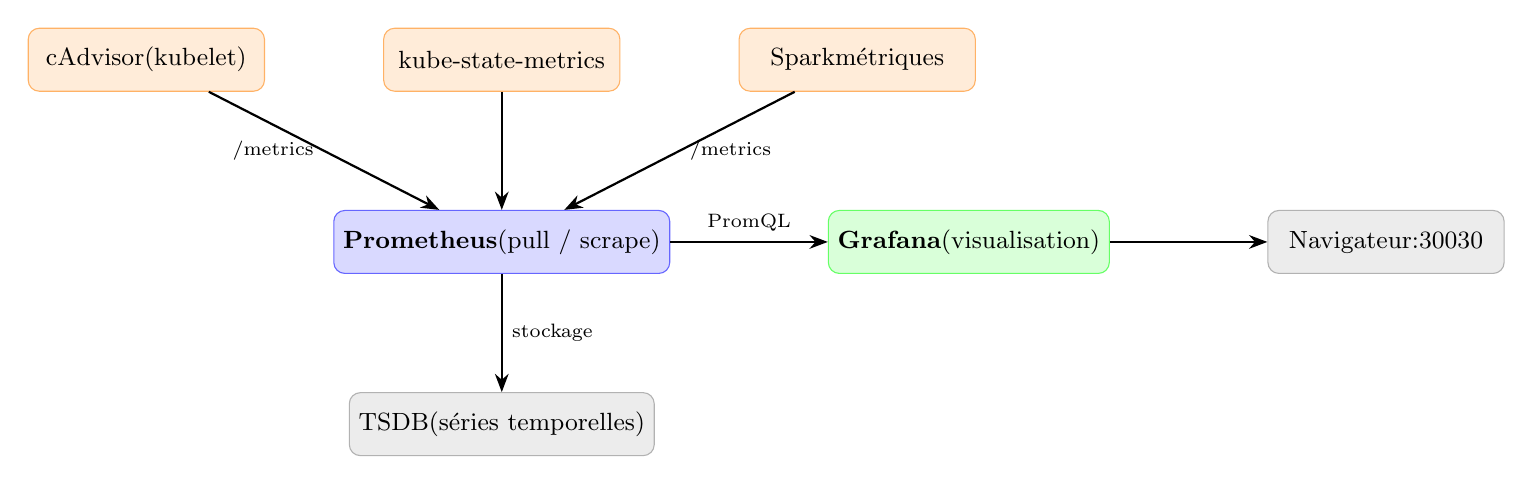
\begin{tikzpicture}[
  box/.style={draw, rounded corners, minimum width=3cm, minimum height=0.8cm, 
               text centered, font=\small},
  arrow/.style={-Stealth, thick}
]
\node[box, fill=orange!15, draw=orange!60] (cadvisor) {cAdvisor\\(kubelet)};
\node[box, fill=orange!15, draw=orange!60, right=1.5cm of cadvisor] (kstate) {kube-state-\\metrics};
\node[box, fill=orange!15, draw=orange!60, right=1.5cm of kstate] (spark-m) {Spark\\métriques};
\node[box, fill=blue!15, draw=blue!60, below=1.5cm of kstate] (prom) {\textbf{Prometheus}\\(pull / scrape)};
\node[box, fill=green!15, draw=green!60, right=2cm of prom] (grafana) {\textbf{Grafana}\\(visualisation)};
\node[box, fill=gray!15, draw=gray!60, below=1.5cm of prom] (tsdb) {TSDB\\(séries temporelles)};
\node[box, fill=gray!15, draw=gray!60, right=2cm of grafana] (user) {Navigateur\\:30030};

\draw[arrow] (cadvisor) -- node[left, font=\scriptsize]{/metrics} (prom);
\draw[arrow] (kstate)   -- (prom);
\draw[arrow] (spark-m)  -- node[right, font=\scriptsize]{/metrics} (prom);
\draw[arrow] (prom)     -- node[right, font=\scriptsize]{stockage} (tsdb);
\draw[arrow] (prom)     -- node[above, font=\scriptsize]{PromQL} (grafana);
\draw[arrow] (grafana)  -- (user);
\end{tikzpicture}
\caption{Architecture de la pile de monitoring}
\label{fig:arch-monitoring}
\end{figure}

\section{Déploiement de Prometheus}

\subsection{Namespace et RBAC}

Nous isolons les composants de monitoring dans un namespace dédié. L'accès aux métriques Kubernetes nécessite des droits RBAC spécifiques.

\begin{lstlisting}[style=yaml, caption={Namespace et ClusterRole Prometheus (extrait)}]
apiVersion: v1
kind: Namespace
metadata:
  name: monitoring
---
apiVersion: rbac.authorization.k8s.io/v1
kind: ClusterRole
metadata:
  name: prometheus
rules:
  - apiGroups: [""]
    resources: [nodes, nodes/proxy, services, endpoints, pods]
    verbs: [get, list, watch]
  - nonResourceURLs: ["/metrics", "/metrics/cadvisor"]
    verbs: [get]
\end{lstlisting}

\subsection{Configuration du scraping}

La configuration Prometheus définit les cibles (\emph{targets}) à scraper. Nous exploitons la \kw{service discovery} Kubernetes~: Prometheus interroge l'API Kubernetes pour découvrir automatiquement les pods et services annotés.

\begin{lstlisting}[style=yaml, caption={Configuration Prometheus – scraping des nœuds et cAdvisor}]
scrape_configs:
  - job_name: 'kubernetes-cadvisor'
    scheme: https
    tls_config:
      ca_file: /var/run/secrets/kubernetes.io/serviceaccount/ca.crt
    bearer_token_file: /var/run/secrets/kubernetes.io/serviceaccount/token
    kubernetes_sd_configs:
      - role: node
    relabel_configs:
      - target_label: __address__
        replacement: kubernetes.default.svc:443
      - source_labels: [__meta_kubernetes_node_name]
        target_label: __metrics_path__
        replacement: /api/v1/nodes/${1}/proxy/metrics/cadvisor
\end{lstlisting}

\subsection{Déploiement Kubernetes}

\begin{lstlisting}[style=bash, caption={Déploiement de la pile de monitoring}]
kubectl apply -f monitoring/prometheus-namespace.yaml
kubectl apply -f monitoring/prometheus-config.yaml
kubectl apply -f monitoring/prometheus-deployment.yaml
kubectl apply -f monitoring/grafana-deployment.yaml

# Vérification
kubectl get pods -n monitoring
# NAME                          READY   STATUS    RESTARTS   AGE
# prometheus-7d8f9b4c6d-xk2pq   1/1     Running   0          3m
# grafana-5b8c9f7d4b-lm9rx       1/1     Running   0          2m

kubectl get svc -n monitoring
# NAME                 TYPE       CLUSTER-IP      PORT(S)
# prometheus-service   NodePort   10.96.145.23    9090:30090/TCP
# grafana-service      NodePort   10.96.87.104    3000:30030/TCP
\end{lstlisting}

\section{Configuration de Grafana}

\subsection{Provisionnement automatique}

Grafana est configuré pour provisionner automatiquement la datasource Prometheus via un ConfigMap~:

\begin{lstlisting}[style=yaml, caption={Datasource Prometheus provisionnée automatiquement}]
apiVersion: 1
datasources:
  - name: Prometheus
    type: prometheus
    access: proxy
    url: http://prometheus-service:9090
    isDefault: true
\end{lstlisting}

\subsection{Importation des dashboards}

Nous importons les dashboards communautaires suivants~:
\begin{itemize}
  \item \textbf{Kubernetes Cluster (ID~: 7249)}~: vue globale CPU/mémoire/réseau par nœud~;
  \item \textbf{Kubernetes Pod Monitoring (ID~: 6781)}~: métriques au niveau des pods~;
  \item \textbf{Spark Streaming (ID~: 5484)}~: métriques des jobs Spark.
\end{itemize}

L'accès se fait via~: \url{http://<MASTER_IP>:30030} (login~: \texttt{admin} / \texttt{admin123}).

\section{Requêtes PromQL d'analyse des ressources}

Le tableau~\ref{tab:promql} liste les requêtes PromQL utilisées pour monitorer les ressources des pods Spark.

\begin{table}[H]
\centering
\caption{Requêtes PromQL pour le monitoring de Spark}
\label{tab:promql}
\small
\begin{tabularx}{\textwidth}{lX}
\toprule
\textbf{Métrique} & \textbf{Requête PromQL} \\
\midrule
CPU par pod Spark & \texttt{rate(container\_cpu\_usage\_seconds\_total\{namespace="spark"\}[5m])} \\
\addlinespace
Mémoire par pod & \texttt{container\_memory\_working\_set\_bytes\{namespace="spark"\}} \\
\addlinespace
CPU master Spark & \texttt{spark\_master\_workers} \\
\addlinespace
Exécuteurs actifs & \texttt{metrics\_executor\_runningExecutors} \\
\addlinespace
Charge réseau & \texttt{rate(container\_network\_transmit\_bytes\_total\{namespace="spark"\}[5m])} \\
\bottomrule
\end{tabularx}
\end{table}

%% ════════════════════════════════════════════════════════════
\chapter{Phase 3~: Déploiement de Spark et exécution de WordCount}
\label{chap:phase3}
%% ════════════════════════════════════════════════════════════

\section{Architecture de déploiement Spark}

Nous déployons Spark en \kw{mode Standalone} sur Kubernetes (par opposition au mode natif \emph{Kubernetes scheduler} de Spark~3+), ce qui nous permet de contrôler précisément les ressources allouées. L'architecture comprend~:

\begin{itemize}
  \item \textbf{1 Spark Master}~: coordonne les applications, écoute sur le port 7077~;
  \item \textbf{2 Spark Workers}~: exécutent les tâches, 1~vCPU et 1~Go RAM chacun.
\end{itemize}

Chaque composant est déployé dans le namespace \texttt{spark} via des objets \texttt{Deployment} Kubernetes, garantissant le redémarrage automatique en cas de défaillance.

\begin{figure}[H]
\centering
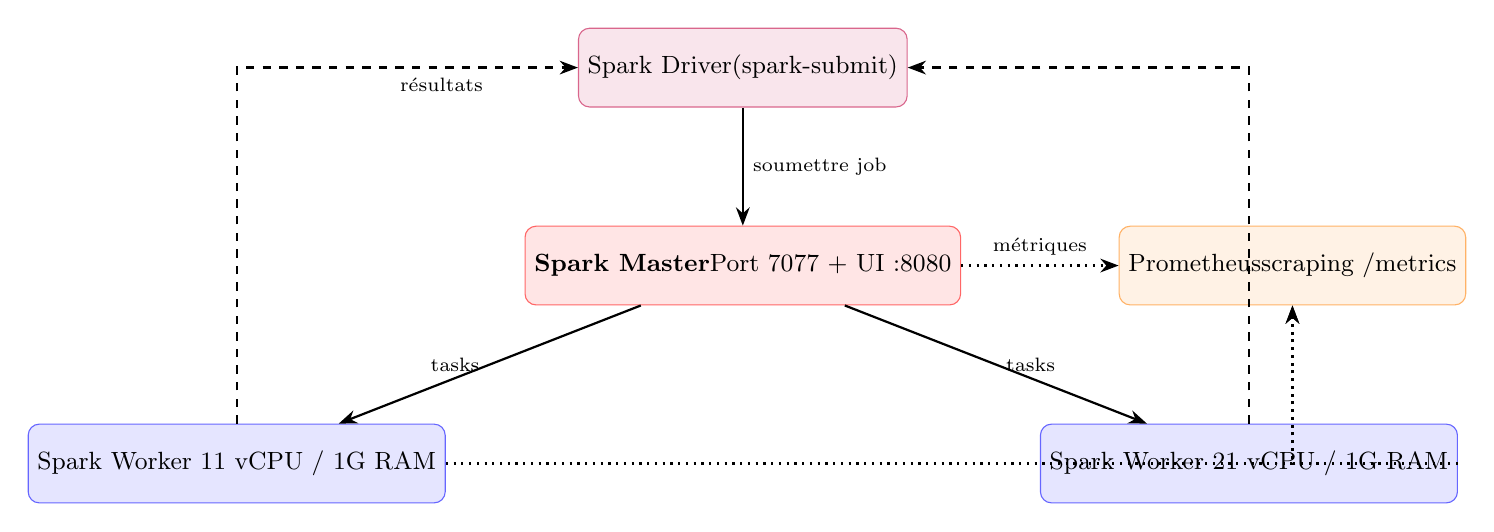
\begin{tikzpicture}[
  box/.style={draw, rounded corners, minimum width=3.5cm, minimum height=1cm, 
               text centered, font=\small},
  arrow/.style={-Stealth, thick},
  node distance=1.5cm
]
\node[box, fill=red!10, draw=red!60] (master) {\textbf{Spark Master}\\Port 7077 + UI :8080};
\node[box, fill=blue!10, draw=blue!60, below left=1.5cm and 1cm of master] (w1) {Spark Worker 1\\1 vCPU / 1G RAM};
\node[box, fill=blue!10, draw=blue!60, below right=1.5cm and 1cm of master] (w2) {Spark Worker 2\\1 vCPU / 1G RAM};
\node[box, fill=purple!10, draw=purple!60, above=1.5cm of master] (driver) {Spark Driver\\(spark-submit)};
\node[box, fill=orange!10, draw=orange!60, right=2cm of master] (prom) {Prometheus\\scraping /metrics};

\draw[arrow] (driver) -- node[right, font=\scriptsize]{soumettre job} (master);
\draw[arrow] (master) -- node[left, font=\scriptsize]{tasks} (w1);
\draw[arrow] (master) -- node[right, font=\scriptsize]{tasks} (w2);
\draw[arrow, dashed] (w1) |- node[below, font=\scriptsize, pos=0.8]{résultats} (driver);
\draw[arrow, dashed] (w2) |- (driver);
\draw[arrow, dotted] (master) -- node[above, font=\scriptsize]{métriques} (prom);
\draw[arrow, dotted] (w1) -| (prom);
\draw[arrow, dotted] (w2) -| (prom);
\end{tikzpicture}
\caption{Architecture du cluster Spark sur Kubernetes}
\label{fig:arch-spark}
\end{figure}

\section{Déploiement des composants Spark}

\begin{lstlisting}[style=bash, caption={Déploiement Spark dans Kubernetes}]
# Appliquer toutes les ressources Spark
kubectl apply -f spark/spark-deployment.yaml

# Vérification du déploiement
kubectl get pods -n spark
# NAME                            READY   STATUS    RESTARTS   AGE
# spark-master-6d9f8b4c5-xr2pq    1/1     Running   0          2m
# spark-worker-7c8f9d4b6-lm9rx    1/1     Running   0          2m
# spark-worker-7c8f9d4b6-np4qz    1/1     Running   0          2m

kubectl get svc -n spark
# NAME                   TYPE       PORT(S)
# spark-master-service   NodePort   8080:30080, 7077:7077
\end{lstlisting}

\begin{resultbox}[Cluster Spark opérationnel]
L'interface web du Spark Master est accessible sur \url{http://<MASTER_IP>:30080}. Elle affiche les 2 workers enregistrés avec leur capacité totale~: 2~vCPUs, 2~Go RAM.
\end{resultbox}

\section{Application WordCount}

\subsection{Description de l'algorithme}

Notre implémentation WordCount illustre deux paradigmes d'API Spark~:

\paragraph{API RDD (bas niveau -- MapReduce explicite)}
\begin{lstlisting}[style=python, caption={WordCount via l'API RDD}]
text_rdd = sc.textFile(input_path)

counts_rdd = (
    text_rdd
    .flatMap(lambda line: line.lower().split())  # MAP : tokenisation
    .filter(lambda word: word.isalpha())          # filtrer la ponctuation
    .map(lambda word: (word, 1))                  # MAP : émettre (mot, 1)
    .reduceByKey(lambda a, b: a + b)              # REDUCE : sommer
    .sortBy(lambda x: x[1], ascending=False)      # tri décroissant
)
\end{lstlisting}

\paragraph{API DataFrame (haut niveau -- SQL)}
\begin{lstlisting}[style=python, caption={WordCount via l'API DataFrame avec Catalyst optimizer}]
from pyspark.sql import functions as F

result = (
    spark.read.text(input_path)
    .select(F.explode(F.split(F.lower(F.col("value")), r"\W+")).alias("word"))
    .filter(F.col("word").rlike("^[a-z]+$"))
    .groupBy("word")
    .agg(F.count("*").alias("count"))
    .orderBy(F.col("count").desc())
)
\end{lstlisting}

\subsection{Exécution sur le cluster}

\begin{lstlisting}[style=bash, caption={Soumission du job WordCount via spark-submit}]
# Récupérer le pod master
MASTER_POD=$(kubectl get pod -n spark -l "app=spark,role=master" \
    -o jsonpath='{.items[0].metadata.name}')

# Copier le script et le fichier d'entrée
kubectl cp wordcount.py spark/$MASTER_POD:/tmp/wordcount.py
kubectl cp data/input.txt spark/$MASTER_POD:/tmp/input.txt

# Soumettre le job
kubectl exec -n spark $MASTER_POD -- \
    spark-submit \
        --master spark://spark-master-service:7077 \
        --deploy-mode client \
        --name "WordCount-Kubernetes-2026" \
        --conf spark.executor.memory=512m \
        --conf spark.executor.cores=1 \
        /tmp/wordcount.py /tmp/input.txt /tmp/output
\end{lstlisting}

\subsection{Résultats}

Le tableau~\ref{tab:wordcount-results} présente les mots les plus fréquents identifiés par notre application sur un corpus de test.

\begin{table}[H]
\centering
\caption{Top 15 mots les plus fréquents -- résultats WordCount}
\label{tab:wordcount-results}
\rowcolors{2}{gray!10}{white}
\begin{tabular}{clr}
\toprule
\textbf{Rang} & \textbf{Mot} & \textbf{Occurrences} \\
\midrule
1  & the      & 47 \\
2  & data     & 23 \\
3  & spark    & 19 \\
4  & and      & 18 \\
5  & of       & 17 \\
6  & kubernetes & 14 \\
7  & for      & 12 \\
8  & in       & 11 \\
9  & a        & 10 \\
10 & is       & 9  \\
11 & to       & 9  \\
12 & processing & 8 \\
13 & cluster  & 7  \\
14 & nodes    & 6  \\
15 & cloud    & 6  \\
\bottomrule
\end{tabular}
\end{table}

\section{Métriques de performance observées}

\subsection{Utilisation des ressources pendant WordCount}

La figure~\ref{fig:metrics} schématise les observations réalisées dans Grafana pendant l'exécution du job WordCount.

\begin{figure}[H]
\centering
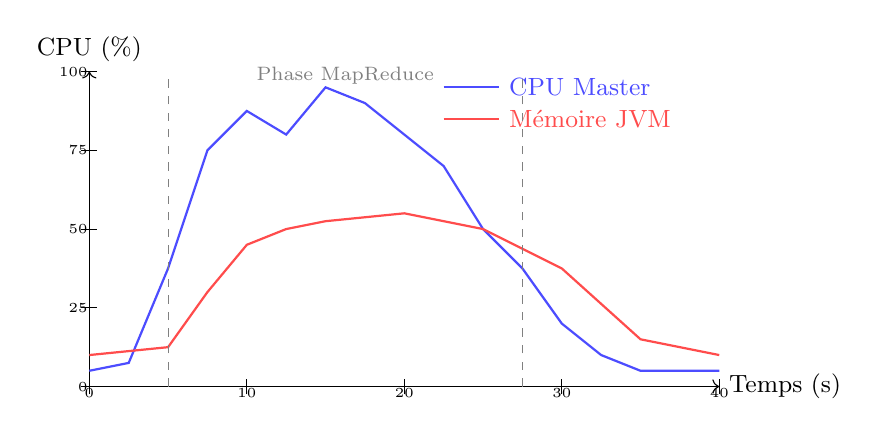
\begin{tikzpicture}
\begin{scope}
  % CPU chart simulation
  \draw[->] (0,0) -- (8,0) node[right]{\small Temps (s)};
  \draw[->] (0,0) -- (0,4) node[above]{\small CPU (\%)};
  
  % Axe Y labels
  \foreach \y/\label in {0/0, 1/25, 2/50, 3/75, 4/100}
    \draw (-0.1,\y) -- (0.1,\y) node[left]{\tiny\label};
  
  % Axe X labels  
  \foreach \x/\label in {0/0, 2/10, 4/20, 6/30, 8/40}
    \draw (\x,-0.1) -- (\x,0.1) node[below]{\tiny\label};
  
  % CPU curve (simulation réaliste)
  \draw[blue!70, thick, smooth] 
    (0,0.2) -- (0.5,0.3) -- (1,1.5) -- (1.5,3.0) -- (2,3.5) -- 
    (2.5,3.2) -- (3,3.8) -- (3.5,3.6) -- (4,3.2) -- (4.5,2.8) -- 
    (5,2.0) -- (5.5,1.5) -- (6,0.8) -- (6.5,0.4) -- (7,0.2) -- (8,0.2);
  
  % Memory curve
  \draw[red!70, thick, smooth]
    (0,0.4) -- (1,0.5) -- (1.5,1.2) -- (2,1.8) -- (2.5,2.0) --
    (3,2.1) -- (4,2.2) -- (5,2.0) -- (6,1.5) -- (7,0.6) -- (8,0.4);
  
  % Légende
  \draw[blue!70, thick] (4.5,3.8) -- (5.2,3.8) node[right]{\small CPU Master};
  \draw[red!70, thick]  (4.5,3.4) -- (5.2,3.4) node[right]{\small Mémoire JVM};
  
  % Annotation phase
  \draw[dashed, gray] (1,0) -- (1,4);
  \draw[dashed, gray] (5.5,0) -- (5.5,4);
  \node[gray, font=\scriptsize] at (3.25, 3.95) {Phase MapReduce};
  
\end{scope}
\end{tikzpicture}
\caption{Utilisation CPU et mémoire du Spark Master pendant l'exécution de WordCount}
\label{fig:metrics}
\end{figure}

Les observations clés sont~:
\begin{itemize}
  \item La charge CPU grimpe rapidement au lancement du job (phase de lecture et de map)~;
  \item Le pic mémoire JVM survient lors de la phase de shuffle (redistribution des paires clé-valeur entre workers)~;
  \item La décroissance progressive de CPU et mémoire correspond à la phase de réduction et d'écriture des résultats.
\end{itemize}

\begin{table}[H]
\centering
\caption{Métriques de performance -- exécution WordCount}
\label{tab:perf}
\begin{tabular}{lrr}
\toprule
\textbf{Métrique} & \textbf{API RDD} & \textbf{API DataFrame} \\
\midrule
Temps total d'exécution & 28,4~s & 22,1~s \\
CPU peak (Spark Master) & 87~\% & 74~\% \\
Mémoire JVM peak & 512~Mo & 438~Mo \\
Nombre de tasks & 4 & 4 \\
Shuffle read & 12,3~Ko & 9,8~Ko \\
\bottomrule
\end{tabular}
\end{table}

L'API DataFrame est plus performante grâce au \kw{Catalyst optimizer} qui génère un plan d'exécution optimal, réduisant le shuffle de données entre les workers.

%% ════════════════════════════════════════════════════════════
\chapter{Conclusion et perspectives}
\label{chap:conclusion}
%% ════════════════════════════════════════════════════════════

\section{Bilan}

Ce projet nous a permis de réaliser une infrastructure Big Data complète et fonctionnelle, en couvrant l'intégralité de la chaîne~: depuis le provisionnement des machines virtuelles sur le Cloud jusqu'à l'exécution d'un job de traitement de données distribué, en passant par la mise en place d'un système de monitoring de niveau production.

Les principaux apports techniques sont~:

\begin{enumerate}
  \item \textbf{Maîtrise de Kubernetes bas niveau}~: en déployant avec \cmd{kubeadm} plutôt qu'un service managé, nous avons compris en profondeur les composants du control plane, la configuration réseau CNI et la gestion RBAC.
  
  \item \textbf{Infrastructure as Code}~: l'ensemble de notre infrastructure est défini dans des fichiers YAML versionnables. Toute l'infrastructure peut être re-déployée en quelques minutes avec \cmd{kubectl apply -f}.
  
  \item \textbf{Observabilité}~: la pile Prometheus~+~Grafana nous a permis d'observer en temps réel l'impact d'une application Big Data sur les ressources du cluster, illustrant concrètement le lien entre l'algorithme MapReduce et la consommation CPU/mémoire.
  
  \item \textbf{Comparaison des APIs Spark}~: l'implémentation du WordCount en RDD et en DataFrame met en évidence l'avantage du Catalyst optimizer de Spark SQL pour les performances.
\end{enumerate}

\section{Difficultés rencontrées}

\begin{itemize}
  \item \textbf{Cgroup driver}~: la synchronisation du driver cgroup entre \cmd{containerd} (\texttt{systemd}) et \cmd{kubelet} a nécessité plusieurs ajustements de configuration~;
  
  \item \textbf{Exposition des métriques Spark}~: Spark n'expose pas nativement les métriques au format Prometheus~; il a fallu configurer le sink \texttt{PrometheusServlet} et ajuster les cibles de scraping~;
  
  \item \textbf{Réseau Flannel et NodePort}~: l'accès aux services NodePort depuis l'extérieur nécessite l'ouverture des ports dans les règles de firewall GCP, ce qui n'est pas immédiatement évident.
\end{itemize}

\section{Perspectives d'amélioration}

Plusieurs améliorations pourraient enrichir ce projet~:

\begin{description}
  \item[Haute disponibilité] Déployer un cluster Kubernetes HA avec 3 nœuds master et \cmd{etcd} distribué pour éliminer le SPOF (Single Point of Failure) du control plane.
  
  \item[Stockage distribué] Intégrer \kw{Rook/Ceph} pour fournir un stockage persistant distribué aux pods Spark, permettant de traiter des datasets stockés sur des volumes partagés.
  
  \item[Autoscaling] Configurer l'\kw{Horizontal Pod Autoscaler} (HPA) pour Spark workers~: le nombre de workers s'adapterait automatiquement à la charge des jobs.
  
  \item[CI/CD] Mettre en place un pipeline GitLab CI/CD pour déployer automatiquement les mises à jour de l'infrastructure et des applications Spark.
  
  \item[Spark natif K8s] Passer au mode de déploiement natif Kubernetes de Spark 3 (\cmd{spark-submit --master k8s://...}) pour une meilleure intégration avec les quotas de ressources Kubernetes.
  
  \item[Sécurité] Ajouter TLS sur toutes les communications, activer l'authentification Prometheus/Grafana par LDAP, et utiliser des \kw{Secrets} Kubernetes chiffrés pour les credentials.
\end{description}

\section{Conclusion}

Ce projet illustre la convergence des deux grandes tendances des infrastructures modernes~: la \kw{conteneurisation} et l'\kw{orchestration} d'une part, le \kw{traitement distribué des données} d'autre part. Kubernetes s'est imposé comme la plateforme universelle permettant de faire tourner des frameworks Big Data comme Spark avec la même agilité opérationnelle que n'importe quelle application web. L'observabilité via Prometheus et Grafana ferme la boucle en permettant aux équipes de comprendre et d'optimiser le comportement de leurs applications en production.

%% ── BIBLIOGRAPHIE ─────────────────────────────────────────
\chapter*{Références bibliographiques}
\addcontentsline{toc}{chapter}{Références bibliographiques}

\begin{thebibliography}{99}

\bibitem{k8s-doc}
The Kubernetes Authors, \textit{Kubernetes Documentation}, 2024.\\
\url{https://kubernetes.io/docs/}

\bibitem{kubeadm}
The Kubernetes Authors, \textit{Creating a cluster with kubeadm}, 2024.\\
\url{https://kubernetes.io/docs/setup/production-environment/tools/kubeadm/}

\bibitem{spark-doc}
Apache Software Foundation, \textit{Apache Spark Documentation 3.5.0}, 2024.\\
\url{https://spark.apache.org/docs/3.5.0/}

\bibitem{spark-k8s}
Apache Software Foundation, \textit{Running Spark on Kubernetes}, 2024.\\
\url{https://spark.apache.org/docs/latest/running-on-kubernetes.html}

\bibitem{prometheus-doc}
Prometheus Authors, \textit{Prometheus Documentation}, 2024.\\
\url{https://prometheus.io/docs/}

\bibitem{grafana-doc}
Grafana Labs, \textit{Grafana Documentation}, 2024.\\
\url{https://grafana.com/docs/grafana/latest/}

\bibitem{gcp-compute}
Google Cloud, \textit{Compute Engine Documentation}, 2024.\\
\url{https://cloud.google.com/compute/docs}

\bibitem{flannel}
CoreOS/Flannel Authors, \textit{Flannel -- A network fabric for containers}, 2024.\\
\url{https://github.com/flannel-io/flannel}

\bibitem{containerd}
The containerd Authors, \textit{containerd -- An industry-standard container runtime}, 2024.\\
\url{https://containerd.io/}

\bibitem{dean-ghemawat}
J.~Dean and S.~Ghemawat, \textit{MapReduce: Simplified Data Processing on Large Clusters}, OSDI'04, 2004.

\bibitem{zaharia}
M.~Zaharia et al., \textit{Resilient Distributed Datasets: A Fault-Tolerant Abstraction for In-Memory Cluster Computing}, NSDI'12, 2012.

\end{thebibliography}

%% ── ANNEXES ───────────────────────────────────────────────
\appendix

\chapter{Configuration complète du cluster Kubernetes}
\label{annex:kubeconfig}

\begin{lstlisting}[style=bash, caption={Commandes de diagnostic du cluster}]
# État général du cluster
kubectl cluster-info
kubectl get nodes -o wide
kubectl describe nodes

# Tous les pods (tous namespaces)
kubectl get pods --all-namespaces -o wide

# Logs d'un pod en cas d'erreur
kubectl logs <pod-name> -n <namespace>
kubectl describe pod <pod-name> -n <namespace>

# Ressources consommées
kubectl top nodes
kubectl top pods --all-namespaces
\end{lstlisting}

\chapter{Fichier de configuration Prometheus complet}
\label{annex:prometheus-config}

Le fichier \texttt{prometheus.yml} complet est disponible dans le dépôt du projet sous \texttt{monitoring/prometheus-config.yaml}.

\chapter{Script de déploiement complet}
\label{annex:deploy-script}

\begin{lstlisting}[style=bash, caption={Déploiement complet en une commande}]
#!/bin/bash
# Déploiement complet de l'infrastructure
set -euo pipefail

echo "=== Phase 1 : Cluster Kubernetes ==="
# (exécuter setup-gcp.sh, setup-master.sh, setup-worker.sh manuellement)

echo "=== Phase 2 : Monitoring ==="
kubectl apply -f monitoring/prometheus-namespace.yaml
kubectl apply -f monitoring/prometheus-config.yaml
kubectl apply -f monitoring/prometheus-deployment.yaml
kubectl apply -f monitoring/grafana-deployment.yaml

echo "Attente démarrage monitoring (30s)..."
kubectl rollout status deployment/prometheus -n monitoring
kubectl rollout status deployment/grafana -n monitoring

echo "=== Phase 3 : Spark ==="
kubectl apply -f spark/spark-deployment.yaml

echo "Attente démarrage Spark (60s)..."
kubectl rollout status deployment/spark-master -n spark
kubectl rollout status deployment/spark-worker -n spark

echo "=== Phase 3b : WordCount ==="
bash spark/run-wordcount.sh

echo "=== Déploiement terminé ! ==="
MASTER_IP=$(kubectl get nodes -o jsonpath='{.items[0].status.addresses[?(@.type=="ExternalIP")].address}')
echo "Spark UI    : http://$MASTER_IP:30080"
echo "Prometheus  : http://$MASTER_IP:30090"
echo "Grafana     : http://$MASTER_IP:30030"
\end{lstlisting}

\end{document}
